\documentclass[12pt]{book}
\usepackage{graphicx}
\usepackage{booktabs}
\usepackage{lab}
\usepackage{fancyhdr}
\usepackage{shadow}
\usepackage{array}
%\usepackage[Sonny]{fncychap}
\usepackage{wrapfig}
\usepackage{multicol}

\newcounter{Lab}
\setcounter{Lab}{-1}

\newcommand{\Labtitle}[1]{
\stepcounter{Lab}
\noindent
%\rule{\linewidth}{1pt}\\[5pt]
\textsc{\large Lab \#\theLab \hfill #1}\\
\rule{\linewidth}{1pt}
\vspace*{-5mm}
}


\pagestyle{fancy}
\fancyhf{}%
\lfoot{\scshape Astronomy 150}%
\cfoot{\theLab\ -- \thepage}%
\rfoot{\scshape The Planets}%
\renewcommand{\headrulewidth}{0pt}

\newcommand{\s}{\rule[-4mm]{0cm}{9mm}}



\makeatletter
\renewcommand{\section}{\@startsection{section}{1}{0pt}%
                       {-0.5\baselineskip}{0.5\baselineskip}%
                       {\normalfont\large\bfseries}%
}
\makeatother

\begin{document}




\setcounter{page}{1}
\setlength{\parindent}{0ex}
\setlength{\baselineskip}{15pt}
\setlength{\parskip}{0.9ex}

\Labtitle{Graphing Tutorial}

\small

\section*{Graphs}

To put it bluntly, I use a boatload of graphs in this class.  You
should be very comfortable with reading and producing graphs.  If you
are not now comfortable, you soon will be.  I have made this little
graph tutorial to define some terms as I use them in class, and to
make sure everybody is on the same page graph-wise.  If you have any
question please ask your TA.

\vskip 3mm

\parbox{9.5cm}{ 
A graph is a chart or drawing that shows the relationship between
changing things.  They are a diagram displaying the relationship
between numbers or amounts. Common graphs use bars, lines, points or
parts of a circle to display data.  Nearly all of the graphs I use in
this class are the classic 2-dimensional X-Y plots.  I will almost
always refer to the horizontal axis as the X-axis and the vertical
axis as the Y-axis (see plot on right).}
\makebox[0.5cm]{}
\raisebox{18mm}{\mbox{\includegraphics[height=50mm,angle=-90]{./images/Graph0.ps}}}

\vskip 3mm

The axes actually have proper names; {\bf ordinate} for the X-axis and
the {\bf abscissa} for the Y-axis.  However, I {\it never} remember
those names so I will not use them.


The two main axes types I use in this class are {\bf linear} and {\bf
  logarithmic}.  Often times I will not mention the types of axes
  displayed, so pay attention.  

A {\bf linear} graph has values that change as you would expect.  In
the example below one point 5 units farther down the X-axis has a value
that is 5 units larger.

\begin{center}
\mbox{\includegraphics[height=10cm,angle=-90]{./images/Graph1.ps}}
\end{center}


A {\bf logarithmic} graph is more complicated.  Generally, the major
division on the graph differ by a power of 10.  For example on the
X-axis below the two points are two major divisions away, but their
values differ by a factor of 100 $=$ (10$^2$).

\begin{center}
\mbox{\includegraphics[height=10cm,angle=-90]{./images/Graph2.ps}}
\end{center}

{N.B.} Many graphs have one axis linear and the other logarithmic.
\\

{\bf Questions}\\

On the back of this page are 4 graphs from this class,  For each of
these graphs you should be able to answer the following questions:

\begin{enumerate}
\item Is the graph linear, logarithmic or a mix?
\item What is being plotted and what is the range of values?
\item What information is being presented in the plot?  Can you explain
the ``message'' of the plot to another person?
\end{enumerate}

\clearpage

\begin{center}
\vfill
\mbox{\includegraphics[height=10cm]{./images/DenvDist.eps}}
\makebox[0.5cm]{}
\mbox{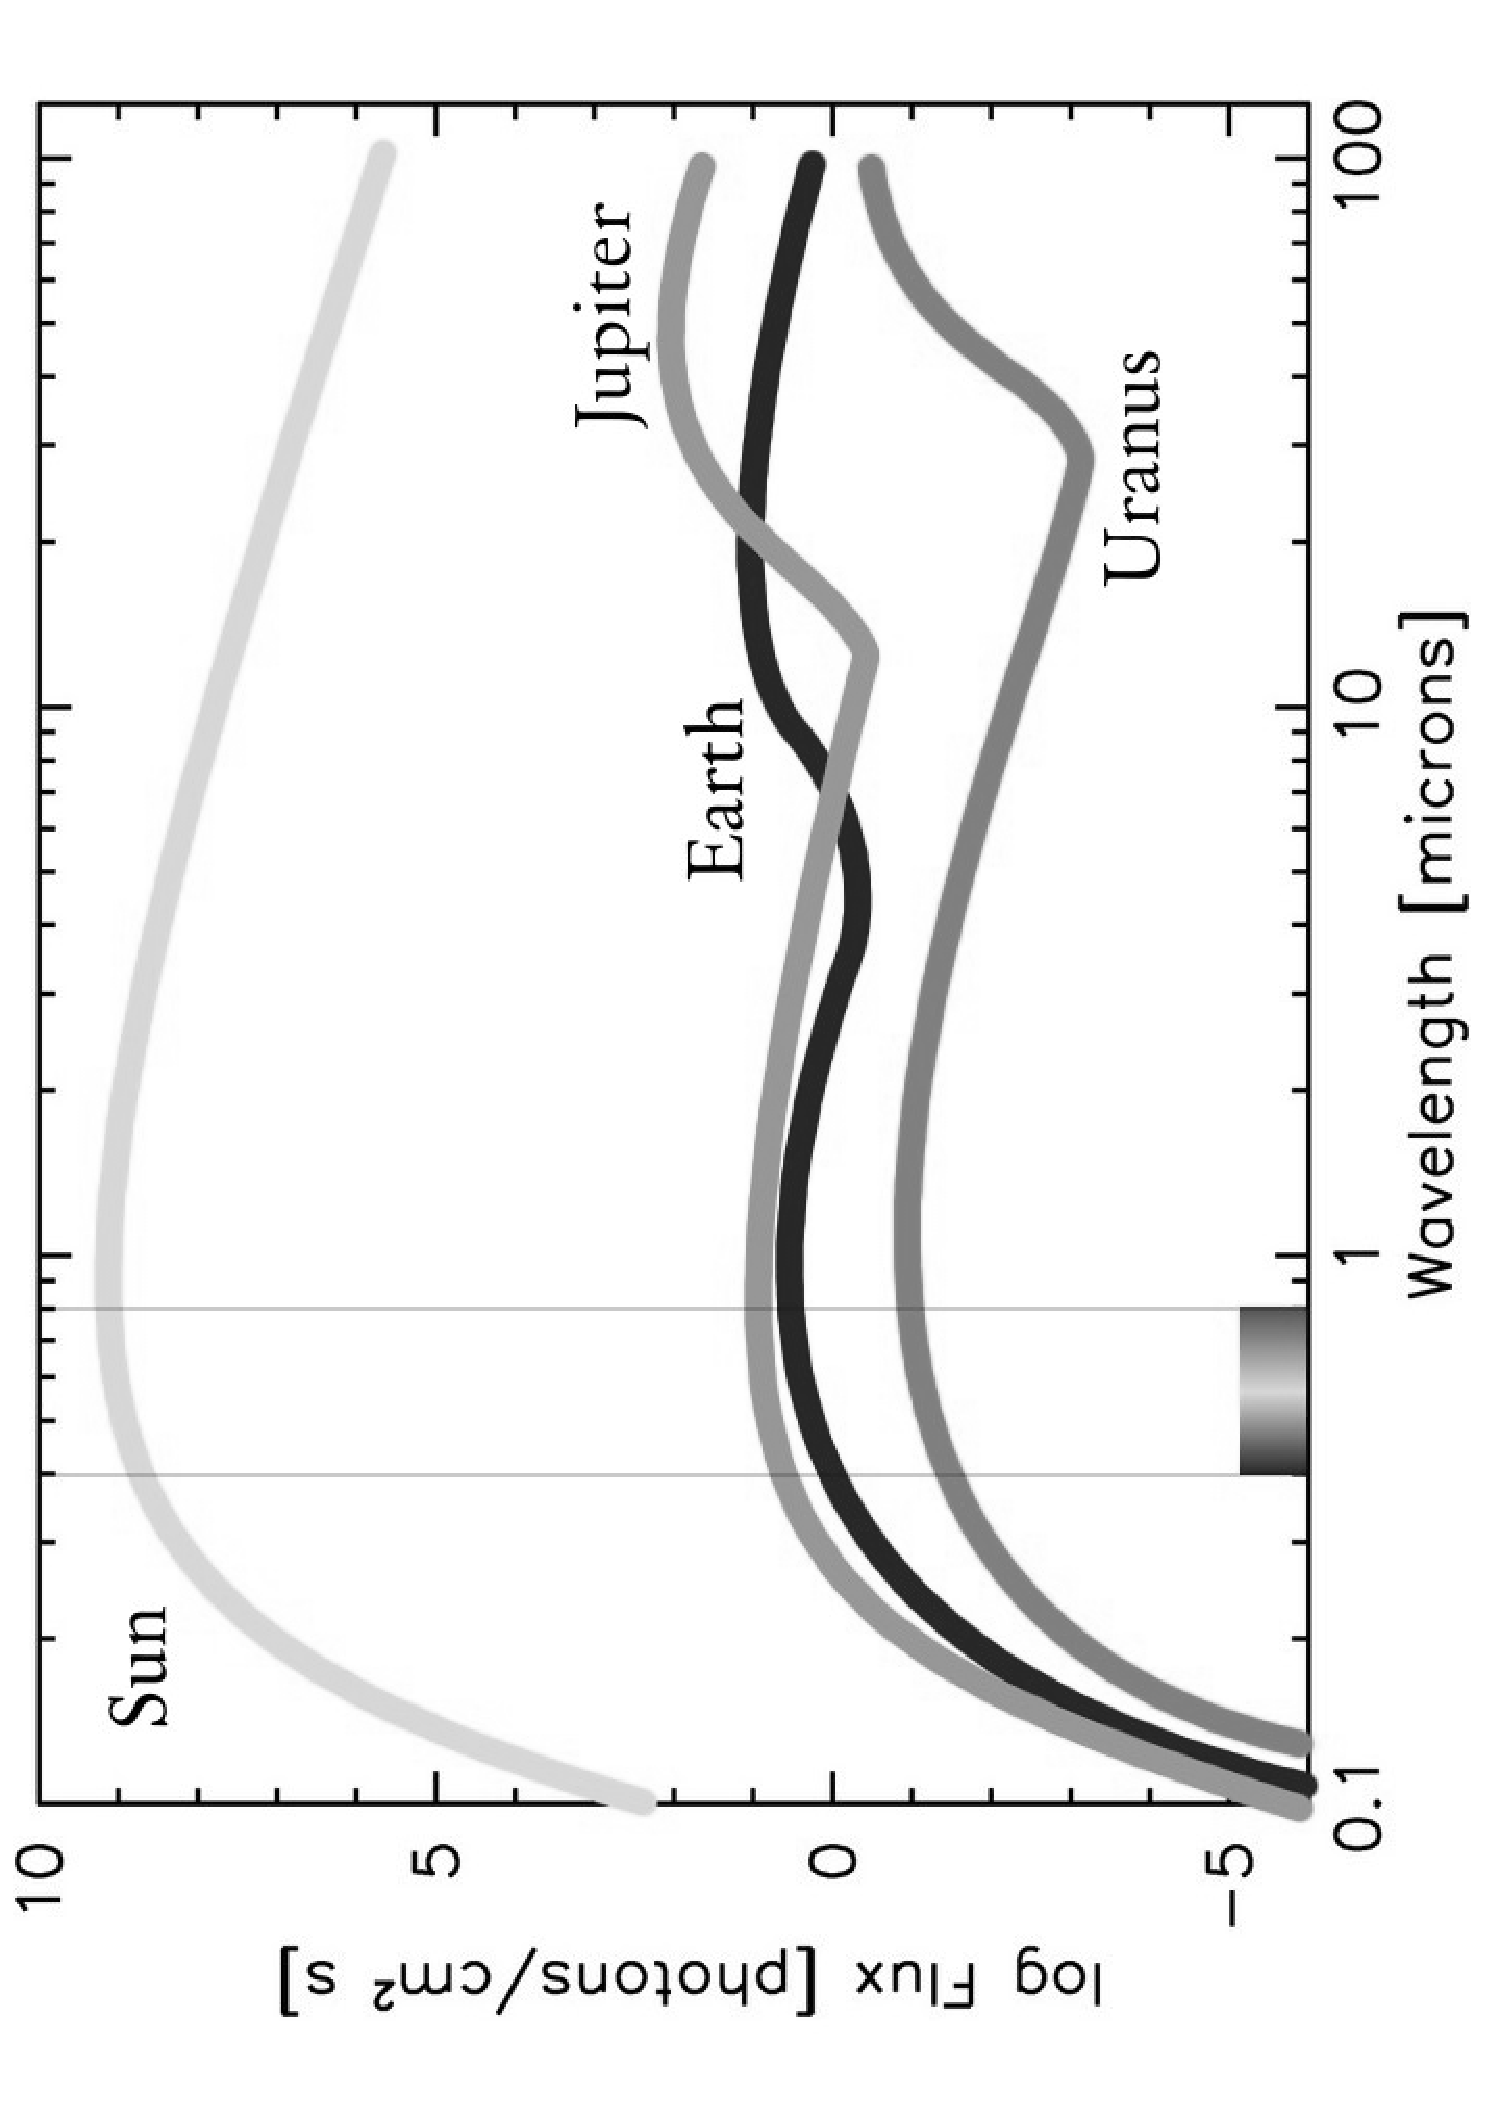
\includegraphics[height=10cm]{./images/SolarFlux.ps}}
\vfill
\mbox{\includegraphics[height=10cm]{./images/UnCompressed.ps}}
\makebox[0.5cm]{}
\mbox{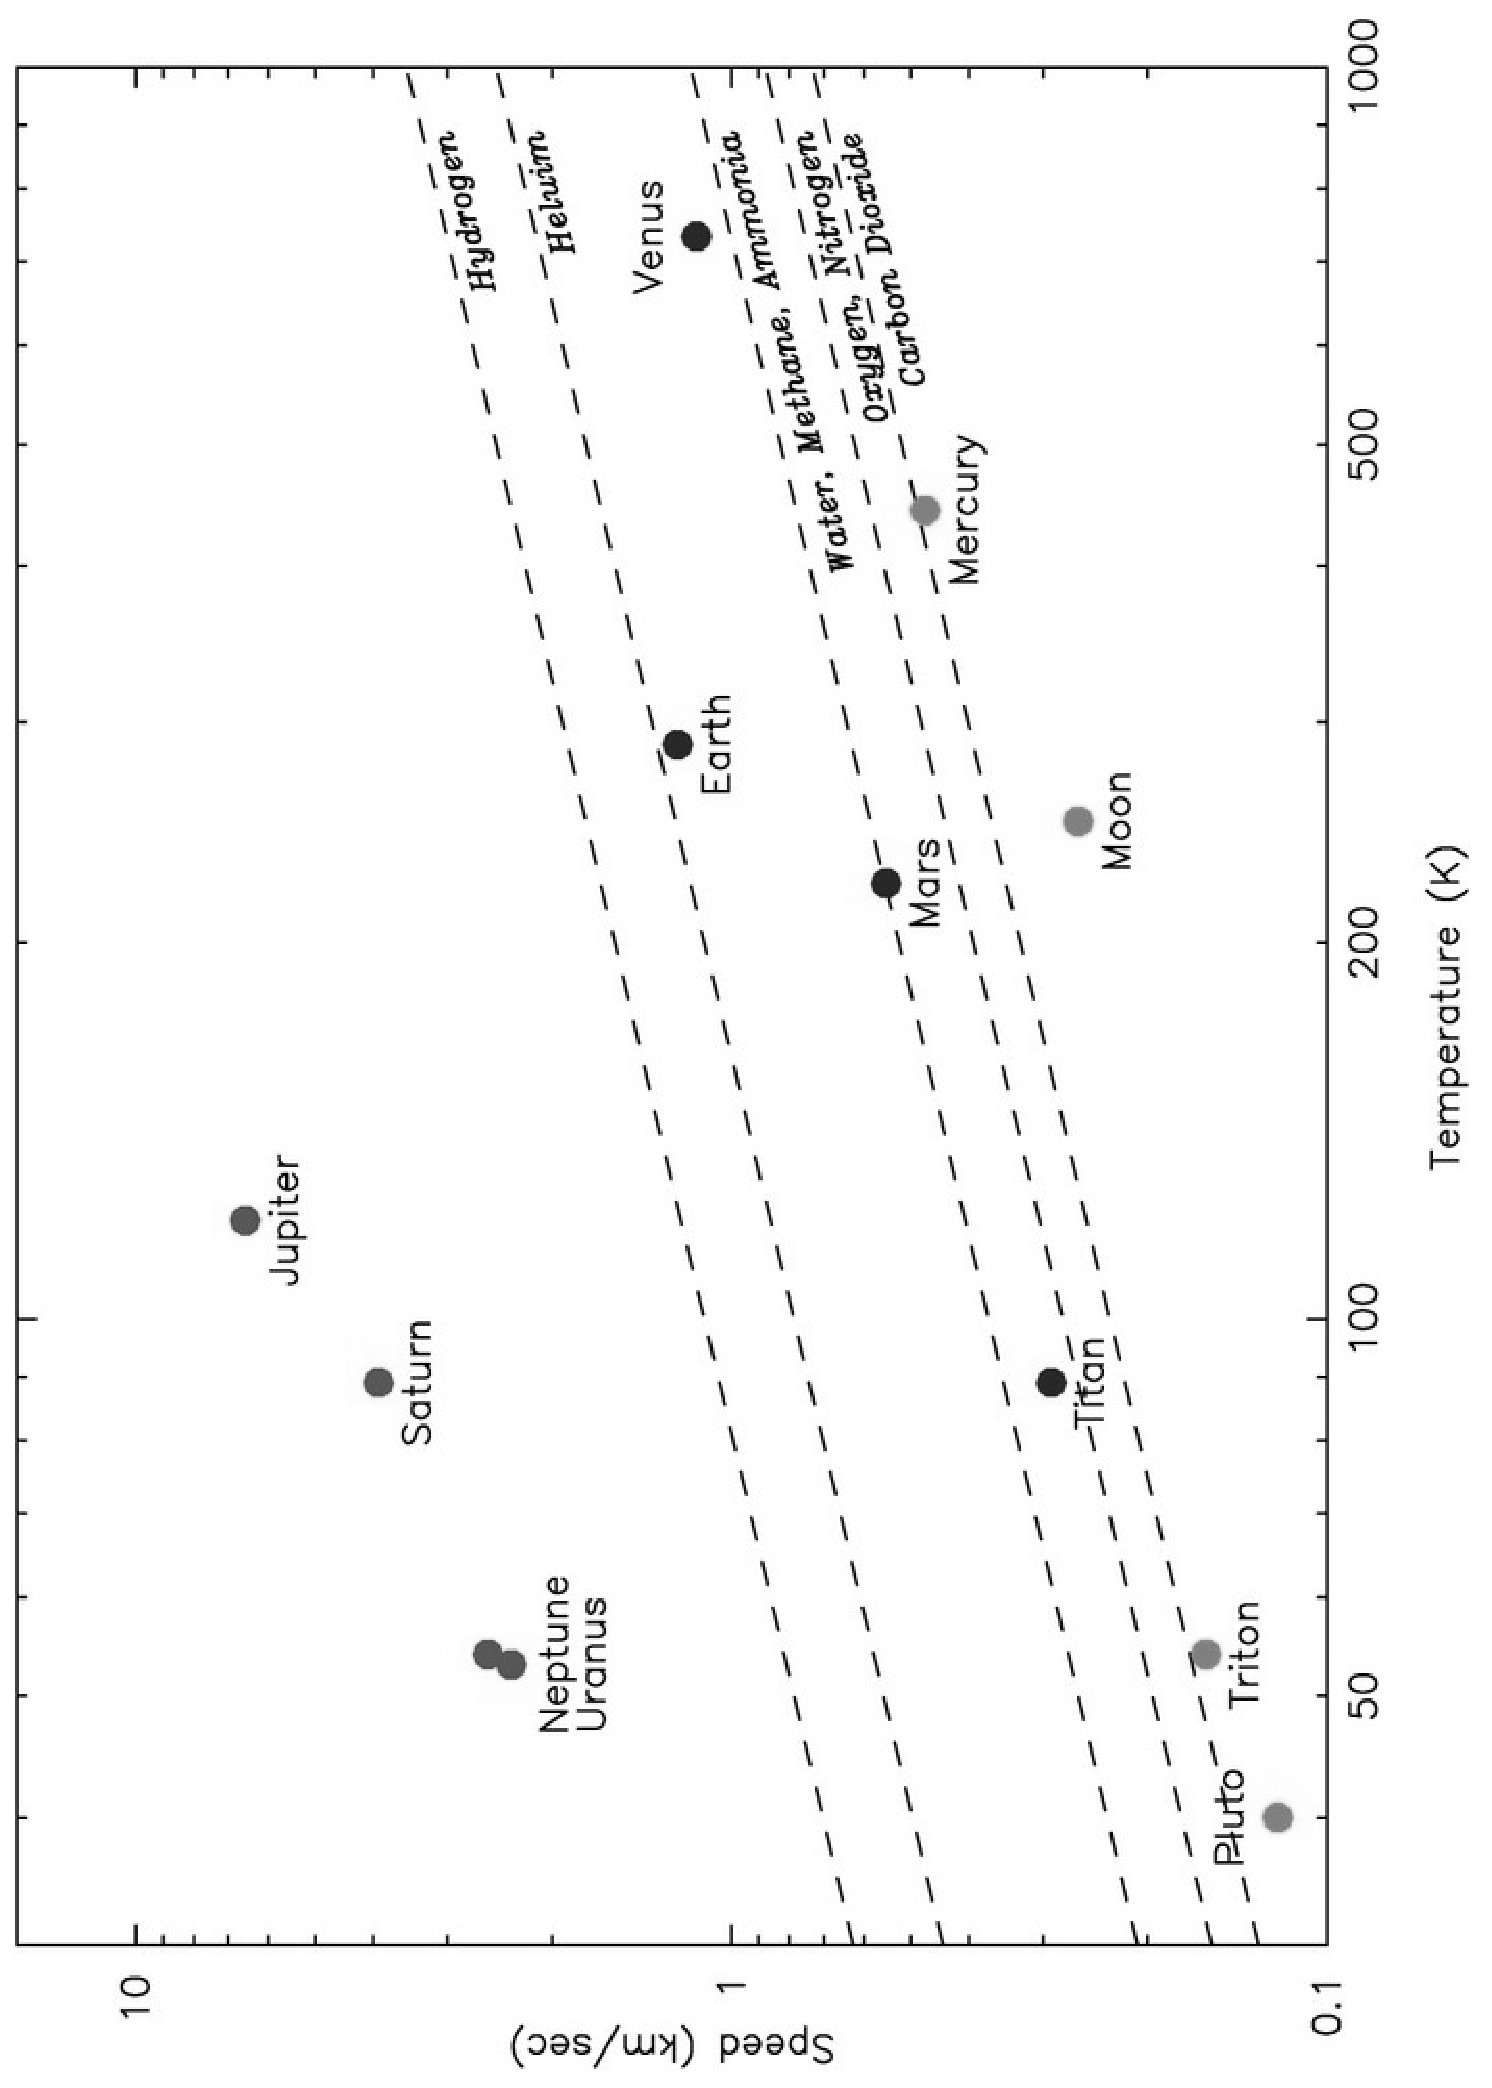
\includegraphics[height=10cm]{./images/Atmos_Escape.ps}}
\vfill
\end{center}

\normalsize
\clearpage

\end{document}
